\chapter{Runtime Monitoring}
\label{chap:RTA}
As described in Section~\ref{sec:runtime}, there is a notable class of systems, referred to as runtime, which are able to handle the complexity and non-compliance of their AI models with safety standards. These systems rely on different solutions to manage their complex algorithms, one of which is known as runtime monitoring. In this scenario, one of the main challenges is to obtain certification when a module is present within the system that does not have deterministic behavior, is very complex to handle in a formal way, and can produce undetectable faults in the system.

One of the most practical solutions to this problem is \textit{runtime assurance} (RTA): we do not try to make the complex module compliant, but instead we want to predict its faulty behavior and, in this case, switch to a safe module. This approach has high modularity: once we have obtained certification for the whole system, we can change the AI module without problems, because if it fails, the safe function enters into action. Another interesting point is that this solution can be applied at any system level (e.g., flight controller and actuation system)~\cite{nagarajan2021astm}.

%%%%%%%%%%%%%%%%%%%%%%%%%%%%%%%%%%%%%%%%%%%%%%%%
\section{Architecture}
The idea we described in the introduction of this chapter is formalized in the \textit{ASTM F3269-17} standard (the latest version is F3269-21, but it must be purchased). In 2017, the Advancing Standards Transforming Market (ASTM) published a guideline to implement this behavior on unmanned aircraft systems. Figure~\ref{fig:RTA_architecture} shows a diagram of the proposed architecture.
\begin{figure}[htbp]
    \centering
    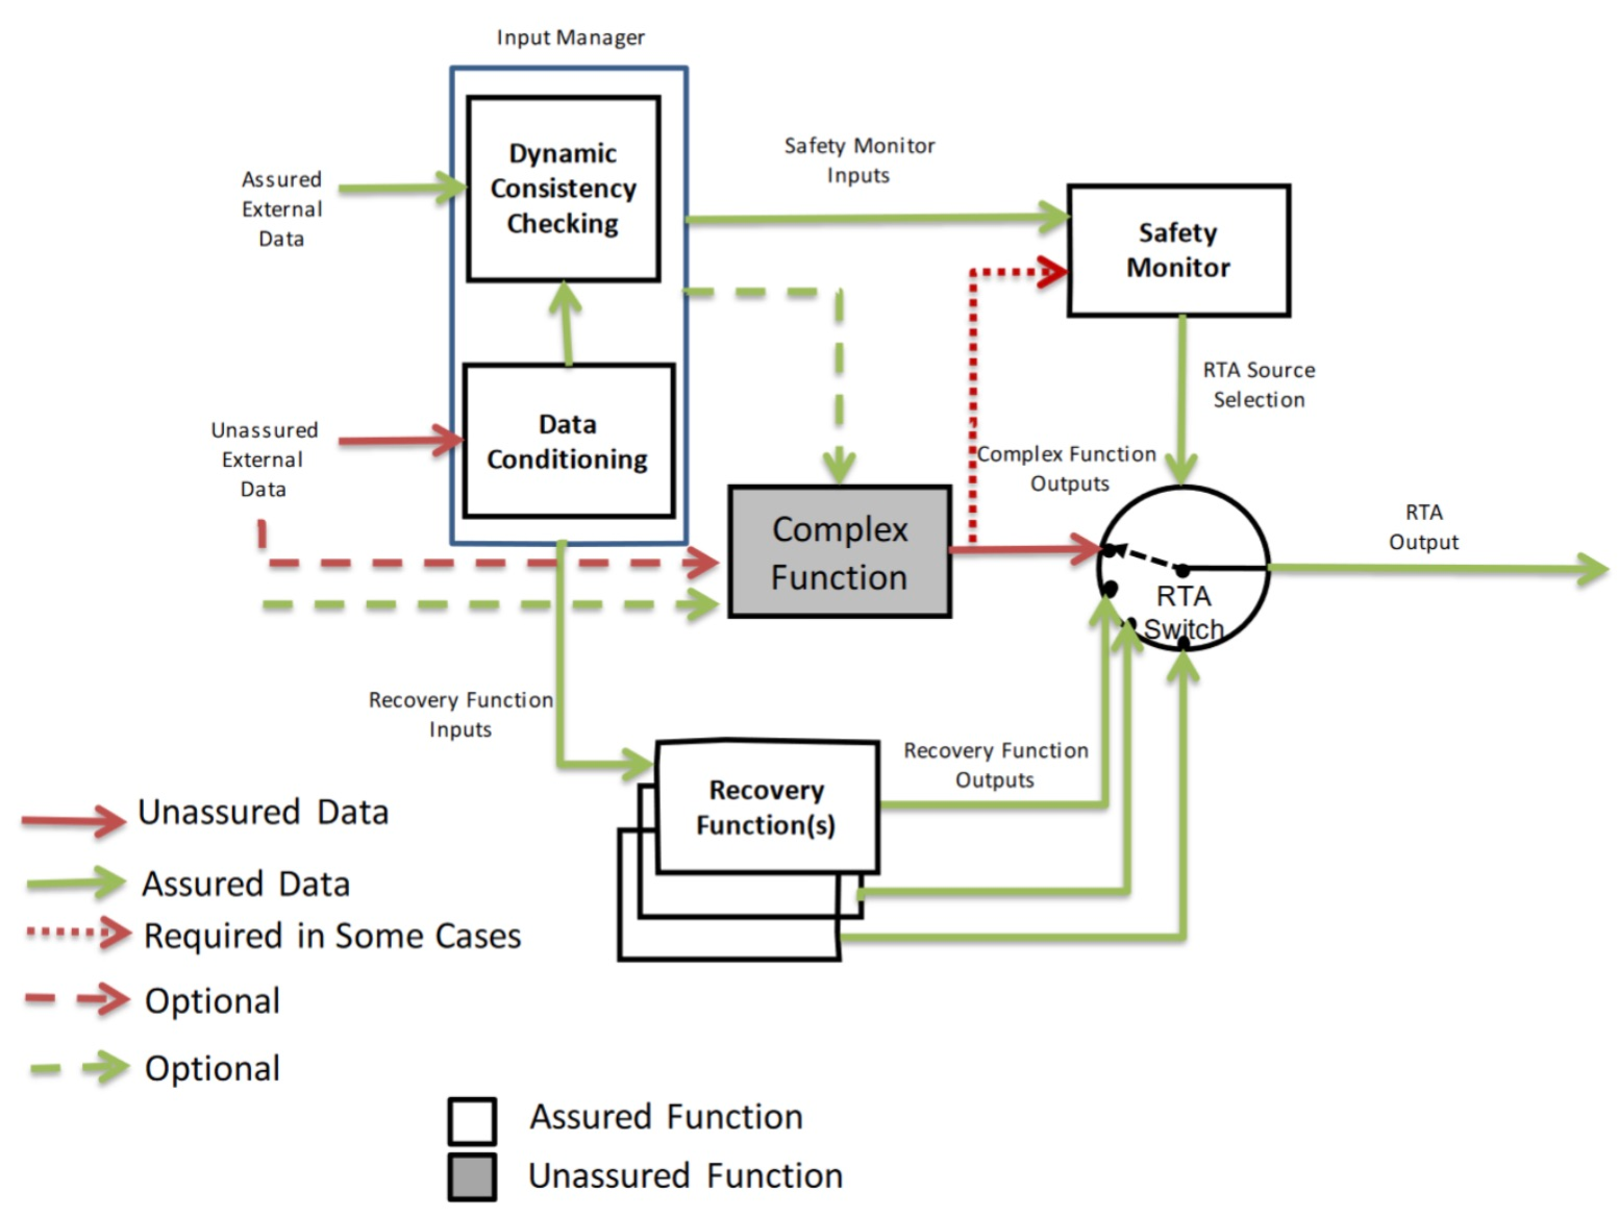
\includegraphics[max width=\textwidth, max height=0.85\textheight, keepaspectratio]{images/3-monitoring/RTA_architecture.pdf}
    \caption{RTA architecture Proposed in ASTM F3269-17~\cite{nagarajan2021astm}.}
    \label{fig:RTA_architecture}
\end{figure}

\myskip

Let's see some terms that are useful to know:
\begin{itemize}
    \item \textbf{Data} \\
        Obviously, data is the information that will be processed by the system. These data can be both assured and unassured: in the first case, we are referring to data that can be used directly by the system; in the second one, we are referring to data that must be validated through the \textbf{Input Manager}.
    \item \textbf{Complex Function} \\
        This is the module that cannot be certified, usually an AI module. This AI component is composed of data pre-processing, inference, and post-processing; furthermore, this component can be implemented with some degree of redundancy, with a voter at the end~\cite{abella2025safexplain}.
    \item \textbf{Recovery Function} \\
        It is an assured function that generates a bounded output to maintain the system in a safe state if the Complex Function fails.
    \item \textbf{Safety Monitor} \\
        The assured function that is responsible for detecting faulty behavior and sending commands to the Switch. This module can observe both the RTA system and the Complex Function; this choice depends on the use case. This monitor can also perform the analysis on the AI module in a hierarchical way (see Figure~\ref{fig:monitor:hierarchical_checker}): the low-level monitor checks for evident errors (e.g., out-of-distribution values) and the high-level monitor checks for more semantic errors~\cite{abella2025safexplain}.
    \item \textbf{Switch} \\
        An assured function that receives the switching command from the Safety Monitor and switches to the Recovery Function.
\end{itemize}
\begin{figure}[htbp]
    \centering
    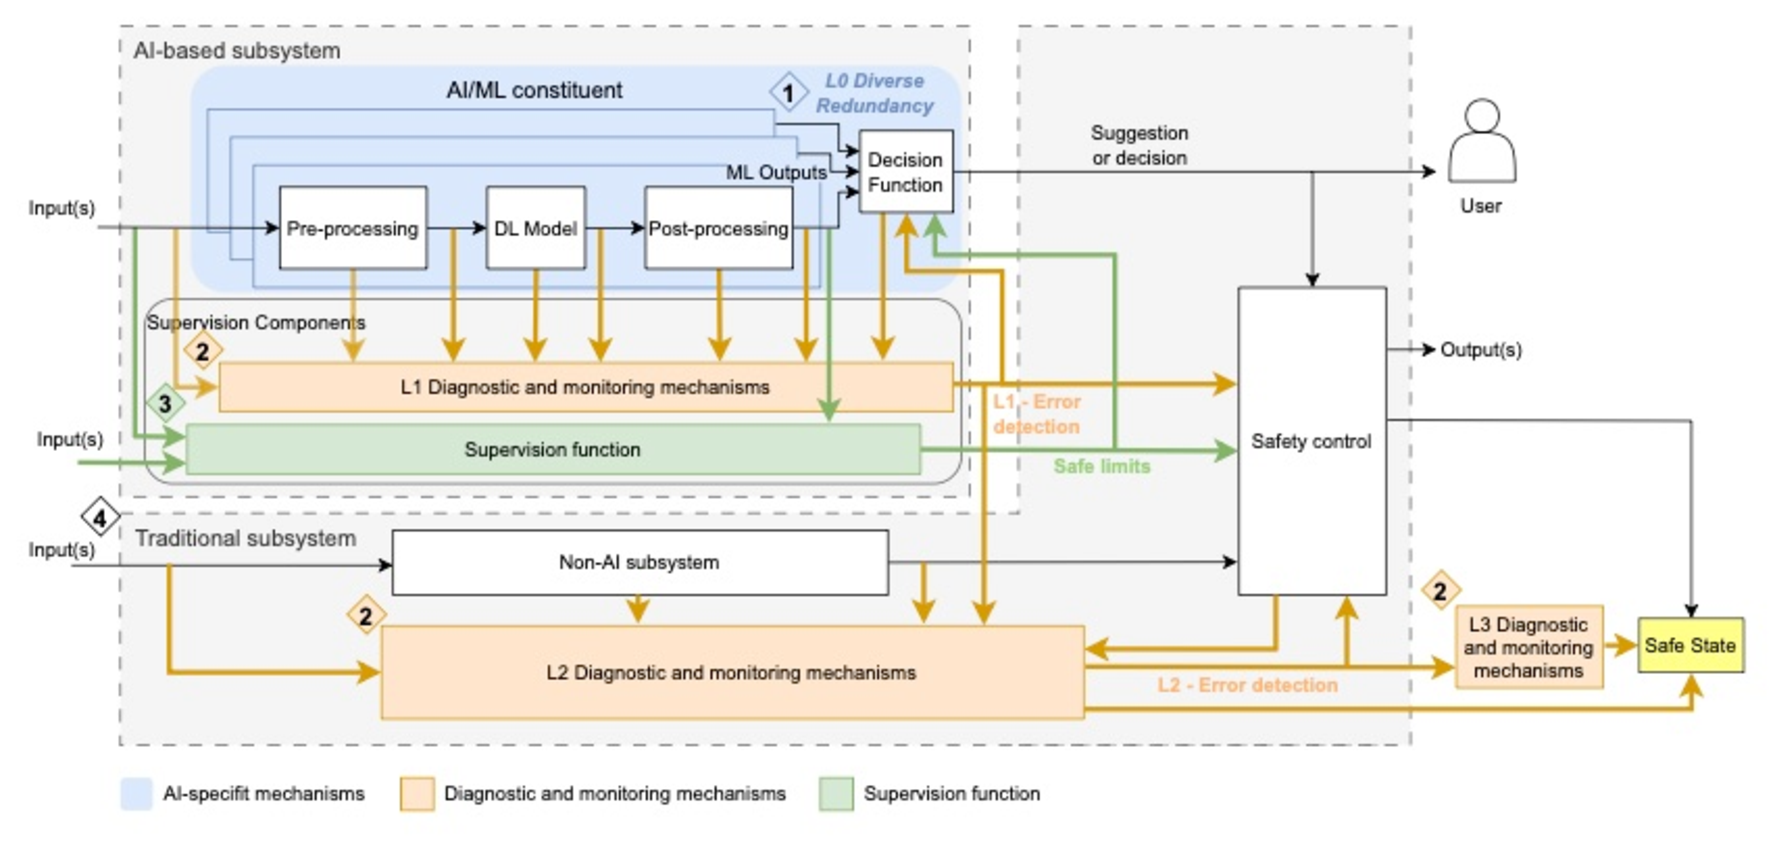
\includegraphics[max width=\textwidth, max height=0.85\textheight, keepaspectratio]{images/3-monitoring/hierarchical_monitor.pdf}
    \caption{RTA architecture with Hierarchical Monitor~\cite{agirre2025functional}.}
    \label{fig:monitor:hierarchical_checker}
\end{figure}

%%%%%%%%%%%%%%%%%%%%%%%%%%%%%%%%%%%%%%%%%%%%%%%%
\section{Coverage}
The coverage concept is fundamental to make the RTA system work. We start from the operational scope of the Complex Function, i.e., from the boundary of the functionality that the Complex Function implements. This scope is analyzed from the viewpoint of all combinations of Safety Monitors and Recovery Functions (see Figure~\ref{fig:monitoring:coverage_gap}): for each operating point (i.e., functionality) of the scope, there must be a monitor capable of detecting the Complex Function's failure and a Recovery Function that maintains the system in a safe state.
\begin{figure}[htbp]
    \centering
    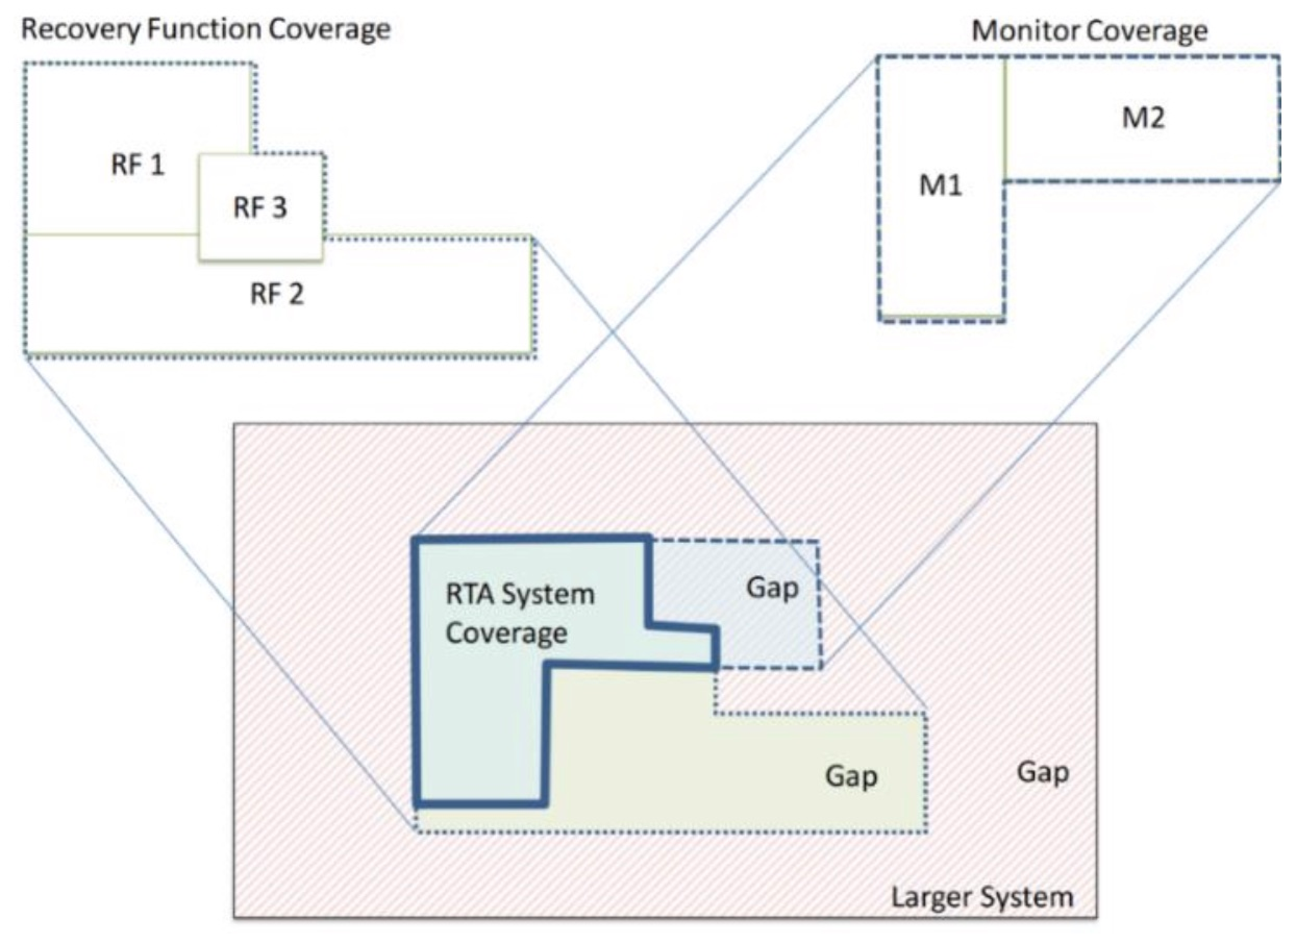
\includegraphics[max width=\textwidth, max height=0.85\textheight, keepaspectratio]{images/3-monitoring/coverage_gap.pdf}
    \caption{Gap in the Monitor and the Recovery Function~\cite{nagarajan2021astm}.}
    \label{fig:monitoring:coverage_gap}
\end{figure}

This concept of coverage leads us to have multiple monitors, where each of them has its own Recovery Function. The choice of which monitor and its relative Recovery Function is performed by a voter, resulting in an architecture similar to the one shown in Figure~\ref{fig:monitor:monitors_voter}.
\begin{figure}[htbp]
    \centering
    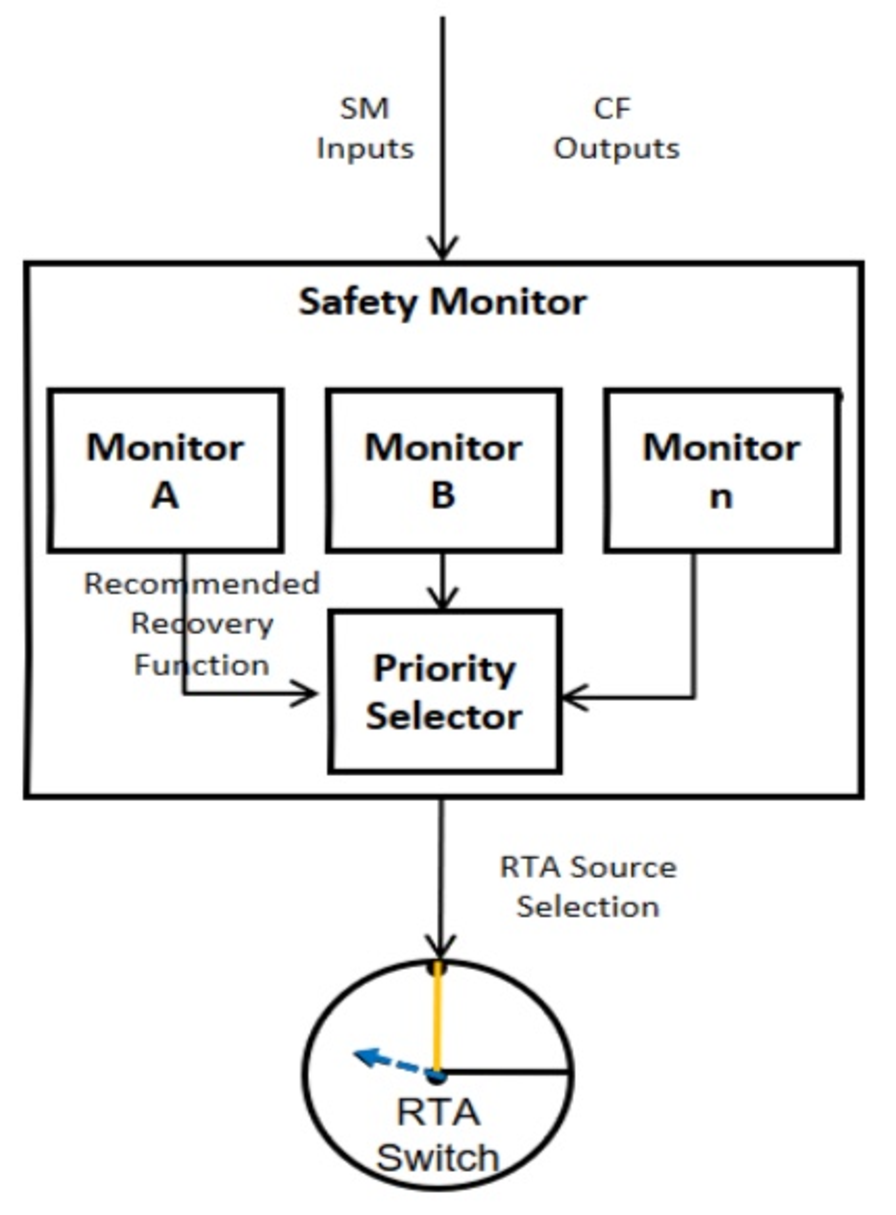
\includegraphics[max width=\textwidth, max height=.85\textheight, keepaspectratio]{images/3-monitoring/monitors_voter.pdf}
    \caption{Voter architecture with multiple Monitors~\cite{nagarajan2021astm}.}
    \label{fig:monitor:monitors_voter}
\end{figure}